\documentclass[10pt,a4paper]{article}
\usepackage[utf8]{inputenc}
\usepackage[T1]{fontenc}
\usepackage[brazilian]{babel}
\usepackage{lmodern}
\usepackage[a4paper,margin=2.2cm]{geometry}
\usepackage{amsmath,amssymb,bm}
\usepackage{graphicx}
\usepackage{booktabs,multirow,tabularx,array}
\usepackage[table]{xcolor}
\usepackage{caption,subcaption}
\usepackage{microtype}
\usepackage{enumitem}
\usepackage{listings}
\usepackage[hidelinks]{hyperref}
\usepackage[brazilian,nameinlink]{cleveref}
\graphicspath{{../results/figs/}}
\captionsetup{font=small,labelfont=bf}
\setlist{nosep,leftmargin=1.4em}
\lstset{basicstyle=\ttfamily\small,columns=fullflexible,frame=single,breaklines=true}
\newcommand{\meanR}{0{,}8162}
\newcommand{\meanG}{0{,}6685}
\newcommand{\meanB}{0{,}6955}
\newcommand{\stdR}{0{,}2152}
\newcommand{\stdG}{0{,}2415}
\newcommand{\stdB}{0{,}1175}
\newcommand{\mlpH}{1024}
\newcommand{\mlpDrop}{0{,}25}
\newcommand{\mlpWD}{0{,}0}
\newcommand{\mlpAcc}{88{,}02}
\newcommand{\mlpBacc}{86{,}54}
\newcommand{\mlpFone}{86{,}38}
\newcommand{\mlpFw}{87{,}99}
\newcommand{\mlpVal}{88{,}08}
\newcommand{\mlpBaccMS}{86{,}62 \pm 0{,}17}
\newcommand{\mlpFoneMS}{86{,}50 \pm 0{,}27}
\newcommand{\mlpParams}{2.419.720}
\newcommand{\mlpTime}{38{,}3}
\newcommand{\mlpEpochs}{41}
\newcommand{\mlpBestEp}{29}
\newcommand{\mlpWeightedWins}{7}
\newcommand{\mlpSeeds}{86{,}54; 86{,}53; 86{,}71; 86{,}90; 86{,}40}
\newcommand{\bBestN}{128}
\newcommand{\bBestK}{7}
\newcommand{\bBestVal}{91{,}87}
\newcommand{\bBestStd}{0{,}08}
\newcommand{\bTotalTime}{70}
\newcommand{\bMinVal}{78{,}32}
\newcommand{\bTimeBest}{211}
\newcommand{\bKspread}{1{,}26}
\newcommand{\bNgain}{9{,}47}
\newcommand{\cAcc}{91{,}52}
\newcommand{\cBacc}{90{,}26}
\newcommand{\cFone}{90{,}52}
\newcommand{\cFw}{91{,}53}
\newcommand{\cVal}{91{,}82}
\newcommand{\cBaccMS}{90{,}06 \pm 0{,}17}
\newcommand{\cFoneMS}{89{,}99 \pm 0{,}39}
\newcommand{\cParams}{219.656}
\newcommand{\cTime}{470{,}1}
\newcommand{\cEpochs}{68}
\newcommand{\cBestEp}{53}
\newcommand{\cNerr}{290}
\newcommand{\cConfErr}{0{,}853}
\newcommand{\cConfOk}{1{,}0000}
\newcommand{\cFracHigh}{41{,}38}
\newcommand{\cPtrue}{0{,}077}
\newcommand{\cTopTwo}{72{,}41}
\newcommand{\cECE}{0{,}0476}
\newcommand{\feCV}{78{,}94 \pm 0{,}93}
\newcommand{\feTest}{78{,}28}
\newcommand{\feFone}{76{,}93}
\newcommand{\feAcc}{79{,}45}
\newcommand{\feTestMS}{78{,}29 \pm 0{,}41}
\newcommand{\feFeatTime}{22}
\newcommand{\feHeadTime}{4{,}4}
\newcommand{\ftCV}{93{,}77 \pm 0{,}36}
\newcommand{\ftEnsBacc}{95{,}16}
\newcommand{\ftEnsAcc}{95{,}18}
\newcommand{\ftEnsFone}{94{,}73}
\newcommand{\ftEnsFw}{95{,}15}
\newcommand{\ftFoldBaccMS}{94{,}40 \pm 0{,}25}
\newcommand{\ftFoldFoneMS}{93{,}75 \pm 0{,}23}
\newcommand{\ftFoldAccMS}{94{,}32 \pm 0{,}20}
\newcommand{\ftParams}{11.180.616}
\newcommand{\ftEpochTime}{60}
\newcommand{\ftFoldTime}{11{,}9}
\newcommand{\ftTotalTime}{59{,}6}
\newcommand{\ftEpochs}{12}
\newcommand{\ftSize}{64}
\newcommand{\ftK}{5}

\makeatletter\newcommand\tabinput[1]{\@@input #1 }\makeatother
\newcommand{\bacc}{\mathrm{BAcc}}
\newcommand{\Fmac}{F_1^{\mathrm{macro}}}

\title{\textbf{IA048 -- Aprendizado de Máquina}\\[2pt]
\large Atividade 3 -- Redes Neurais Artificiais: MLPs e CNNs\\
\normalsize Reconhecimento de células sanguíneas periféricas (BloodMNIST)}
\author{Guilherme Braga do Vale (RA 300875) \and Omar Martín Gálvez Chachayma (RA 300894)}
\date{Turma A -- 2º semestre de 2026 \\ Prof. Levy Boccato}

\begin{document}
\maketitle

\begin{abstract}
\noindent Este relatório documenta o projeto, a seleção de hiperparâmetros e a avaliação de três famílias de
classificadores para as oito classes da BloodMNIST ($28\times28\times3$): (a) MLP de uma camada oculta;
(b)--(c) CNN ``artesanal'' de uma única camada convolucional, com varredura em grade do número e do tamanho
dos kernels; (d) ResNet-18 pré-treinada na ImageNet-1k, adaptada por \emph{transfer learning} e treinada com
validação cruzada estratificada de 5 partições. Todas as escolhas são tomadas exclusivamente com dados de
validação; o conjunto de teste oficial (3.421 imagens) é usado uma única vez por modelo final. No teste, a
acurácia balanceada (BAcc) foi de $\mlpBacc\%$ (MLP, $\mlpParams$ parâmetros), $\cBacc\%$ (CNN simples,
$\cParams$ parâmetros) e $\ftEnsBacc\%$ (comitê de ResNet-18 ajustadas finamente). O código-fonte
completo (\texttt{.py}) acompanha este documento e reproduz todas as tabelas e figuras.
\end{abstract}

%======================================================================
\section{Dados, protocolo experimental e métricas}\label{sec:proto}
%======================================================================
\paragraph{Base e partições.} Utilizou-se o arquivo oficial \texttt{bloodmnist.npz} do MedMNIST v2
\cite{yang2021,acevedo2020} na resolução $28\times28$ (MD5 \texttt{7053d0359d879ad8a5505303e11de1dc},
conferido). Foram mantidas as partições \emph{oficiais} de treino/validação/teste, o que torna os resultados
comparáveis à literatura e elimina qualquer escolha arbitrária de divisão. A \cref{tab:dist} mostra a
distribuição de classes: o desbalanceamento é moderado (razão máxima $\approx 2{,}7$ entre neutrófilos e
linfócitos/basófilos) e idêntico, em proporção, nas três partições (estratificação oficial). A
\cref{fig:samples} ilustra amostras de cada classe.

\begin{table}[h]
\centering\small
\caption{Número de imagens por classe e partição (BloodMNIST, partições oficiais).}\label{tab:dist}
\begin{tabular}{lrrrrrrrr|r}
\toprule
 & BAS & EOS & ERB & IG & LIN & MON & NEU & PLT & Total\\\midrule
Treino    & 852 & 2181 & 1085 & 2026 & 849 & 993 & 2330 & 1643 & 11.959\\
Validação & 122 & 312 & 155 & 290 & 122 & 143 & 333 & 235 & 1.712\\
Teste     & 244 & 624 & 311 & 579 & 243 & 284 & 666 & 470 & 3.421\\\bottomrule
\end{tabular}\\[2pt]
{\footnotesize BAS: basófilo; EOS: eosinófilo; ERB: eritroblasto; IG: granulócito imaturo; LIN: linfócito; MON: monócito; NEU: neutrófilo; PLT: plaqueta.}
\end{table}

\begin{figure}[h]
\centering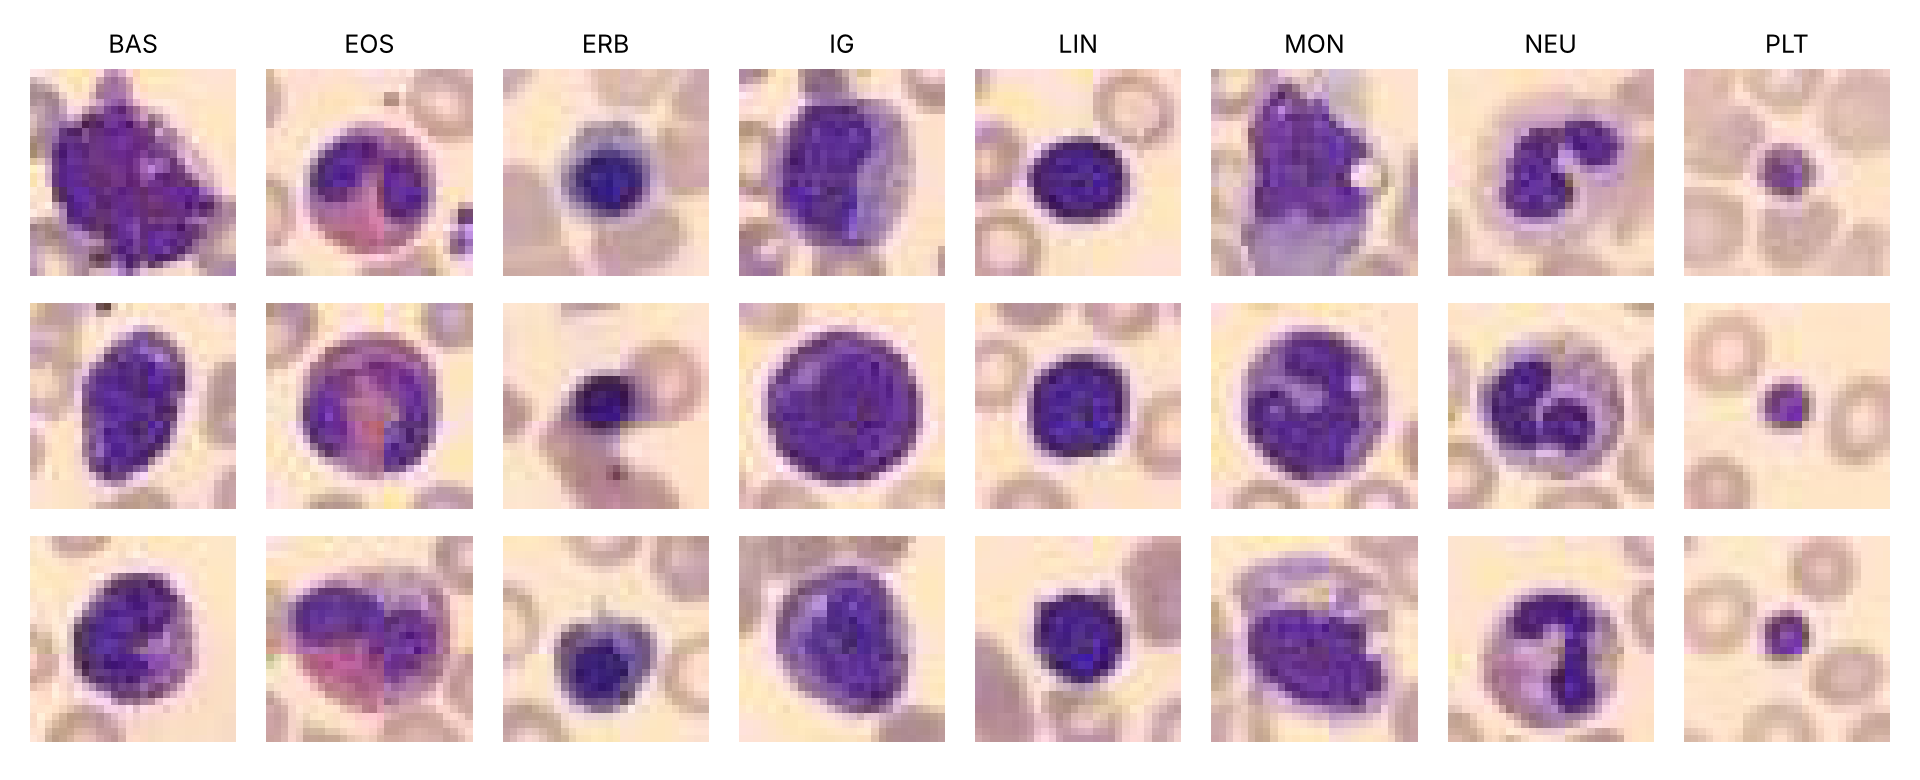
\includegraphics[width=.72\linewidth]{f_samples.png}
\caption{Três amostras aleatórias (semente 0) de cada classe do conjunto de treino.}\label{fig:samples}
\end{figure}

\paragraph{Pré-processamento.} Os pixels são levados a $[0,1]$ e padronizados por canal,
$\tilde x_c = (x_c-\mu_c)/\sigma_c$, com $\bm\mu=(\meanR,\meanG,\meanB)$ e
$\bm\sigma=(\stdR,\stdG,\stdB)$ estimados \emph{somente no treino} (evita vazamento de informação de
validação/teste). Para a ResNet-18 usam-se as estatísticas da ImageNet, pois os pesos pré-treinados
pressupõem essa normalização (\cref{sec:tl}). Não se aplicou aumentação de dados em (a)--(c), para que a
comparação de arquiteturas isole o efeito da arquitetura em si; em (d) ela é parte do protocolo de
ajuste fino.

\paragraph{Métricas.} Sendo $C=8$, $\mathrm{TP}_c$, $\mathrm{FP}_c$, $\mathrm{FN}_c$ as contagens da classe $c$ e
$R_c=\mathrm{TP}_c/(\mathrm{TP}_c+\mathrm{FN}_c)$, $P_c=\mathrm{TP}_c/(\mathrm{TP}_c+\mathrm{FP}_c)$:
\begin{equation}
\bacc=\frac{1}{C}\sum_{c=1}^{C}R_c,\qquad
\Fmac=\frac{1}{C}\sum_{c=1}^{C}\frac{2P_cR_c}{P_c+R_c},\qquad
F_1^{\mathrm{pond}}=\sum_{c}\frac{N_c}{N}\,F_{1,c}.
\end{equation}
A BAcc é o \textbf{critério único de seleção de modelos} (na validação), pois é insensível à prevalência das
classes; reporta-se também a acurácia global (Acc), a $\Fmac$ (``F1-medida'' pedida no enunciado, que pesa
igualmente todas as classes) e a $F_1^{\mathrm{pond}}$. As matrizes de confusão exibem contagens e a fração
por linha (revocação).

\paragraph{Treinamento (comum a todos os modelos).} Entropia cruzada com \emph{ponderação por classe}
$w_c=N/(C\,N_c)$ (justificada empiricamente na \cref{sec:mlp}), que torna o risco empírico um estimador do
risco sob distribuição uniforme de classes --- coerente com a BAcc. Otimizador Adam
($\eta_0=10^{-3}$, $\beta=(0{,}9;\,0{,}999)$), mini-lotes de 128, \texttt{ReduceLROnPlateau} (fator 0,5)
sobre a BAcc de validação, e \emph{early stopping}: o treinamento é interrompido após $p$ épocas sem melhora
da BAcc de validação e os pesos da melhor época são restaurados. Inicialização padrão do PyTorch
(Kaiming-uniforme).

\paragraph{Reprodutibilidade e plataforma.} Sementes fixas (\texttt{random}, NumPy, PyTorch) em cada
treinamento; sementes distintas para varredura e avaliação final. Software: Python 3, PyTorch 2.15 (CPU),
scikit-learn. \textbf{Hardware: CPU com 2 núcleos virtuais, sem GPU}; todos os tempos são de relógio
(\emph{wall-clock}), medidos no mesmo ambiente e portanto comparáveis entre si, mas não em valor absoluto com
execuções em GPU.

%======================================================================
\section{(a) MLP com uma camada intermediária}\label{sec:mlp}
%======================================================================
\paragraph{Arquitetura.} A imagem padronizada é vetorizada ($\mathbf x\in\mathbb R^{2352}$) e
\begin{equation}
\hat{\mathbf p}=\mathrm{softmax}\!\big(\mathbf W_2\,\mathrm{Dropout}_p\big(f(\mathrm{BN}(\mathbf W_1\mathbf x+\mathbf b_1))\big)+\mathbf b_2\big),
\quad \mathbf W_1\in\mathbb R^{H\times2352},\ \mathbf W_2\in\mathbb R^{8\times H}.
\end{equation}
A normalização em lote (BN) após a projeção afim condiciona melhor o problema (pré-ativações com escala
controlada independentemente de $H$) e acelera a convergência; ela não acrescenta camadas intermediárias,
apenas $2H$ parâmetros afins. O número de parâmetros é $2353H+2H+8(H+1)$.

\paragraph{Seleção em duas etapas.} Uma grade completa seria desnecessariamente custosa; adotou-se busca
coordenada, sempre pela BAcc de validação (semente 0, $\le80$ épocas, paciência 12):
\begin{enumerate}
\item \textbf{Etapa 1} -- largura $H\in\{64,\dots,2048\}$ $\times$ ativação $f\in\{\mathrm{ReLU},\tanh\}$, com
$p=0{,}25$, sem \emph{weight decay}, perda ponderada (\cref{tab:mlp1});
\item \textbf{Etapa 2} -- com o melhor $(H,f)$: dropout $p\in\{0;0{,}25;0{,}5\}$ $\times$ \emph{weight decay}
$\lambda\in\{0;10^{-4};10^{-3}\}$ $\times$ perda ponderada ou não (\cref{tab:mlp2}).
\end{enumerate}

\begin{table}[h]
\centering\small
\begin{minipage}[t]{.44\linewidth}\centering
\caption{Etapa 1: BAcc de validação (\%).}\label{tab:mlp1}
\begin{tabular}{rccr}\toprule
$H$ & ReLU & $\tanh$ & Parâmetros\\\midrule
\tabinput{gen/tab_mlp_stage1.tex}
\bottomrule\end{tabular}
\end{minipage}\hfill
\begin{minipage}[t]{.52\linewidth}\centering
\caption{Etapa 2 ($H=\mlpH$, ReLU): BAcc de validação (\%).}\label{tab:mlp2}
\begin{tabular}{cccc}\toprule
$p$ & $\lambda$ & CE ponderada & CE padrão\\\midrule
\tabinput{gen/tab_mlp_stage2.tex}
\bottomrule\end{tabular}
\end{minipage}
\end{table}

\paragraph{Análise da seleção.} (i) A BAcc cresce monotonicamente com $H$ até $H=1024$ e satura
($H=2048$ não melhora e custa $\approx 3\times$ mais tempo): a capacidade deixa de ser o gargalo e passa a
dominar a ausência de vieses indutivos espaciais. (ii) ReLU supera $\tanh$ em todas as larguras (0,45--1,55 p.p.),
consistente com a menor saturação de gradientes. (iii) A perda ponderada venceu em $\mlpWeightedWins$ das 9
combinações $(p,\lambda)$, confirmando a escolha usada em todo o trabalho. (iv) Dropout 0,25 foi
melhor que 0 e 0,5; \emph{weight decay} teve efeito marginal (diferenças $\lesssim0{,}7$ p.p., da ordem da variância
entre sementes), de modo que se preferiu a configuração mais simples ($\lambda=\mlpWD$).

\paragraph{Modelo final.} $H=\mlpH$, ReLU, BN, $p=\mlpDrop$, $\lambda=\mlpWD$, CE ponderada,
$\mlpParams$ parâmetros. Foi retreinado com 5 sementes (100--104); a ``melhor versão'' é a de maior
BAcc de \emph{validação} ($\mlpVal\%$), avaliada uma única vez no teste. A variabilidade entre sementes
é reportada para indicar a significância das diferenças.

\begin{table}[h]
\centering\small
\caption{MLP -- desempenho no conjunto de teste.}\label{tab:mlpres}
\begin{tabular}{lcccc}\toprule
 & Acc (\%) & BAcc (\%) & $\Fmac$ (\%) & $F_1^{\mathrm{pond}}$ (\%)\\\midrule
Melhor versão (sel. por validação) & \mlpAcc & \mlpBacc & \mlpFone & \mlpFw\\
5 sementes (média $\pm$ desvio) & -- & $\mlpBaccMS$ & $\mlpFoneMS$ & --\\\bottomrule
\end{tabular}
\end{table}

\begin{figure}[h]
\centering
\begin{subfigure}{.46\linewidth}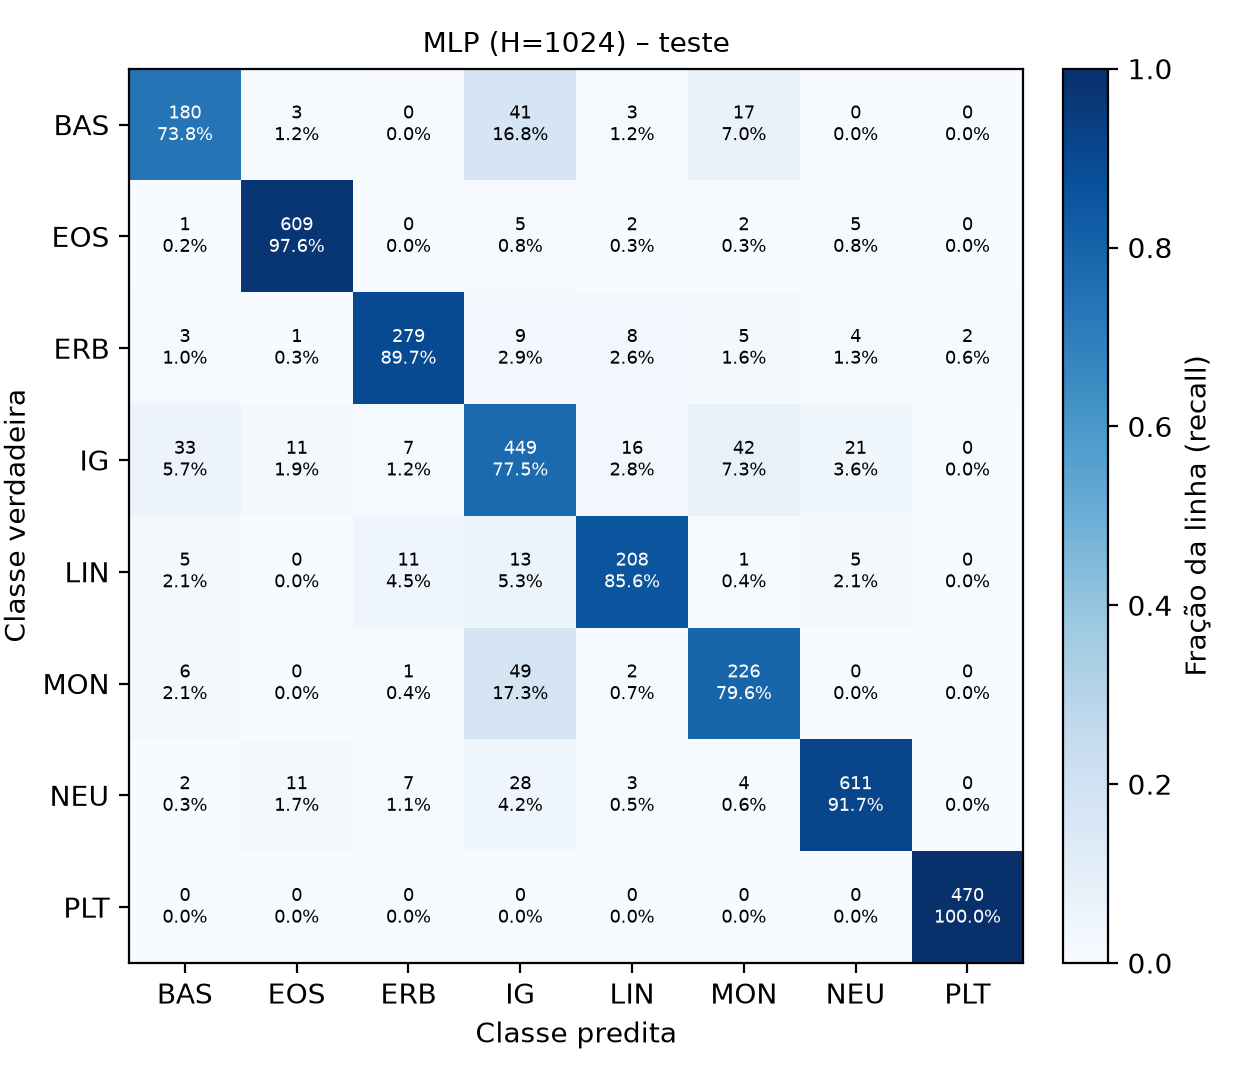
\includegraphics[width=\linewidth]{a_mlp_cm.png}\caption{Matriz de confusão (teste).}\end{subfigure}\hfill
\begin{subfigure}{.52\linewidth}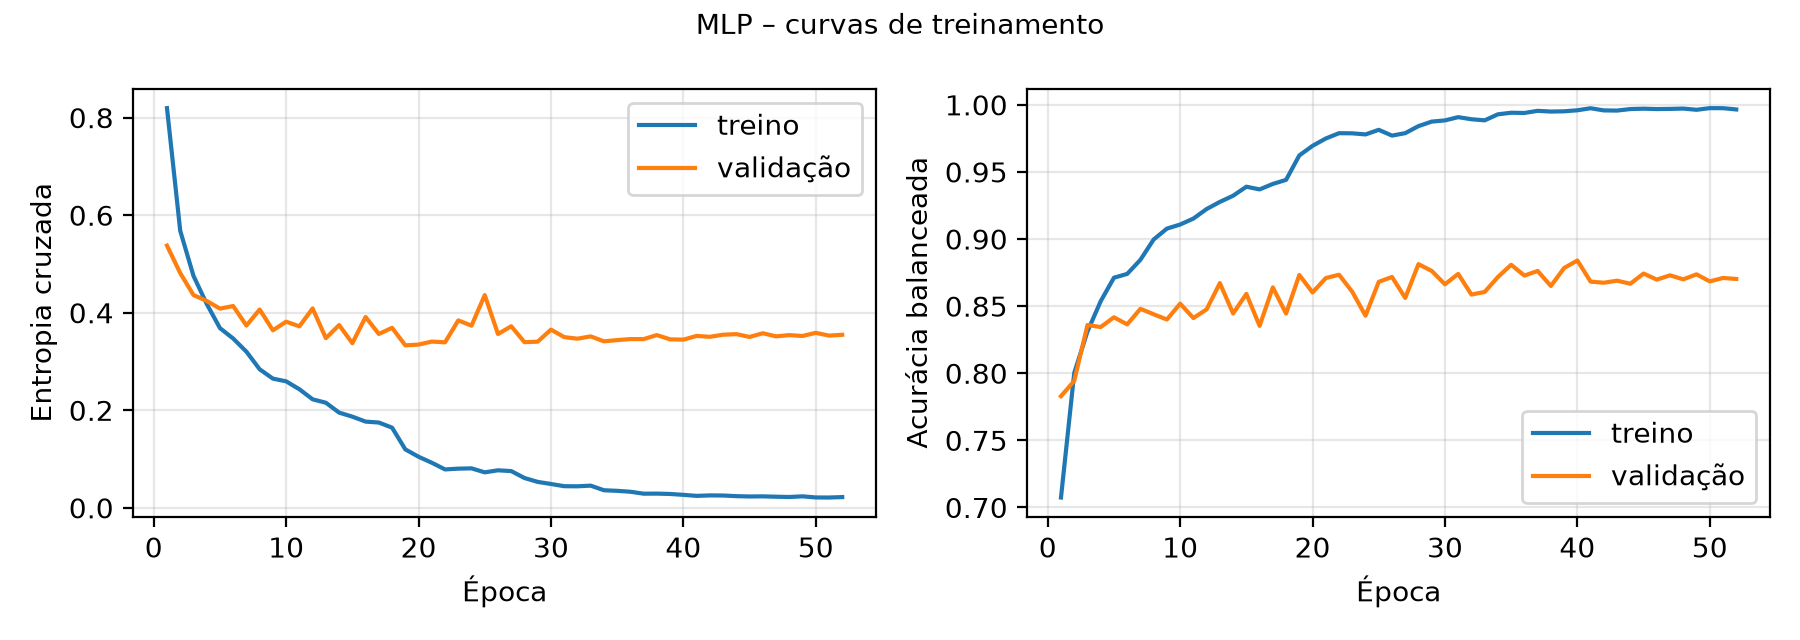
\includegraphics[width=\linewidth]{a_mlp_hist.png}\caption{Curvas de treinamento (perda e BAcc).}\end{subfigure}
\caption{MLP selecionada ($H=\mlpH$). O treinamento parou na época \mlpEpochs{} (melhor época: \mlpBestEp).}\label{fig:mlp}
\end{figure}

\paragraph{Discussão.} BAcc $=\mlpBacc\%$ e $\Fmac=\mlpFone\%$ (\cref{tab:mlpres}), com desvio entre
sementes de apenas $\sim$0,2 p.p. A matriz de confusão (\cref{fig:mlp}) revela a estrutura dos erros:
plaquetas (100\%) e eosinófilos (96,6\%) são quase perfeitamente separadas --- as primeiras por tamanho e
textura muito distintos, os segundos pela coloração alaranjada dos grânulos, que é informação essencialmente
\emph{cromática} e portanto acessível mesmo sem estrutura espacial. Os erros concentram-se no triângulo
\textbf{BAS--IG--MON}: 13,9\% dos basófilos e 15,1\% dos monócitos são atribuídos a granulócitos imaturos, e
os IG (72,5\% de revocação) espalham-se por BAS, MON e NEU. Biologicamente, ``granulócito imaturo'' agrupa
promielócitos, mielócitos e metamielócitos \cite{acevedo2020}, morfologias intermediárias entre as demais
classes; discriminá-las exige relações espaciais entre núcleo e citoplasma (forma/lobulação do núcleo), que
uma MLP, por não ter invariância a translação nem compartilhamento de pesos, só pode aprender
``decorando'' posições de pixels. As curvas de treinamento mostram BAcc de treino continuando a subir enquanto
a de validação estabiliza --- sobreajuste controlado pelo \emph{early stopping}.

%======================================================================
\section{(b) CNN simples: varredura do número e do tamanho dos kernels}\label{sec:cnnb}
%======================================================================
\paragraph{Arquitetura (exatamente a pedida).}
$\mathrm{Conv}_{3\to n}^{k\times k}$ (passo 1, \emph{padding} ``same'' $=\lfloor k/2\rfloor$) $\to$ ReLU $\to$
MaxPool $2\times2$ (passo 2) $\to$ vetorização ($n\cdot14\cdot14$) $\to$ camada densa $\to$ softmax (8 saídas).
O \emph{padding} ``same'' mantém o mapa em $28\times28$ para qualquer $k$, de modo que o tamanho da entrada da
camada de saída depende apenas de $n$ e a comparação entre $k$ não é contaminada por perda de bordas.
Max-pooling foi escolhido por conferir invariância local a pequenas translações e reter as respostas mais
fortes de cada detector. Número de parâmetros: $n(3k^2+1)+8(196n+1)$ --- dominado pela camada de saída
($1568n$), enquanto a convolução contribui com $3nk^2$.

\paragraph{Protocolo.} Grade completa $n\in\{2,4,8,16,32,64,128\}$ $\times$ $k\in\{3,5,7,9,11\}$
(35 configurações), \textbf{2 sementes por ponto} (70 treinamentos, $\approx\bTotalTime$ min de CPU), mesmo
treinamento da \cref{sec:proto} com $\lambda=10^{-4}$, $\le60$ épocas e paciência 8. Reporta-se média $\pm$
desvio da melhor BAcc de validação. A faixa de $n$ cobre de um extremo sub-paramétrico (2 mapas) à saturação;
a de $k$ vai do kernel mínimo usual (3) a 11, i.e., $\approx40\%$ da largura da imagem --- o diâmetro típico
de uma célula na imagem $28\times28$ é de 15--20 pixels.

\begin{table}[h]
\centering\footnotesize
\setlength{\tabcolsep}{3.5pt}
\caption{BAcc de validação (\%, média $\pm$ desvio em 2 sementes) da CNN simples. Em negrito, o melhor ponto.}\label{tab:sweep}
\begin{tabular}{c|ccccccc}\toprule
$k\backslash n$ & 2 & 4 & 8 & 16 & 32 & 64 & 128\\\midrule
\tabinput{gen/tab_cnn_sweep.tex}
\bottomrule\end{tabular}
\end{table}

\begin{figure}[h]
\centering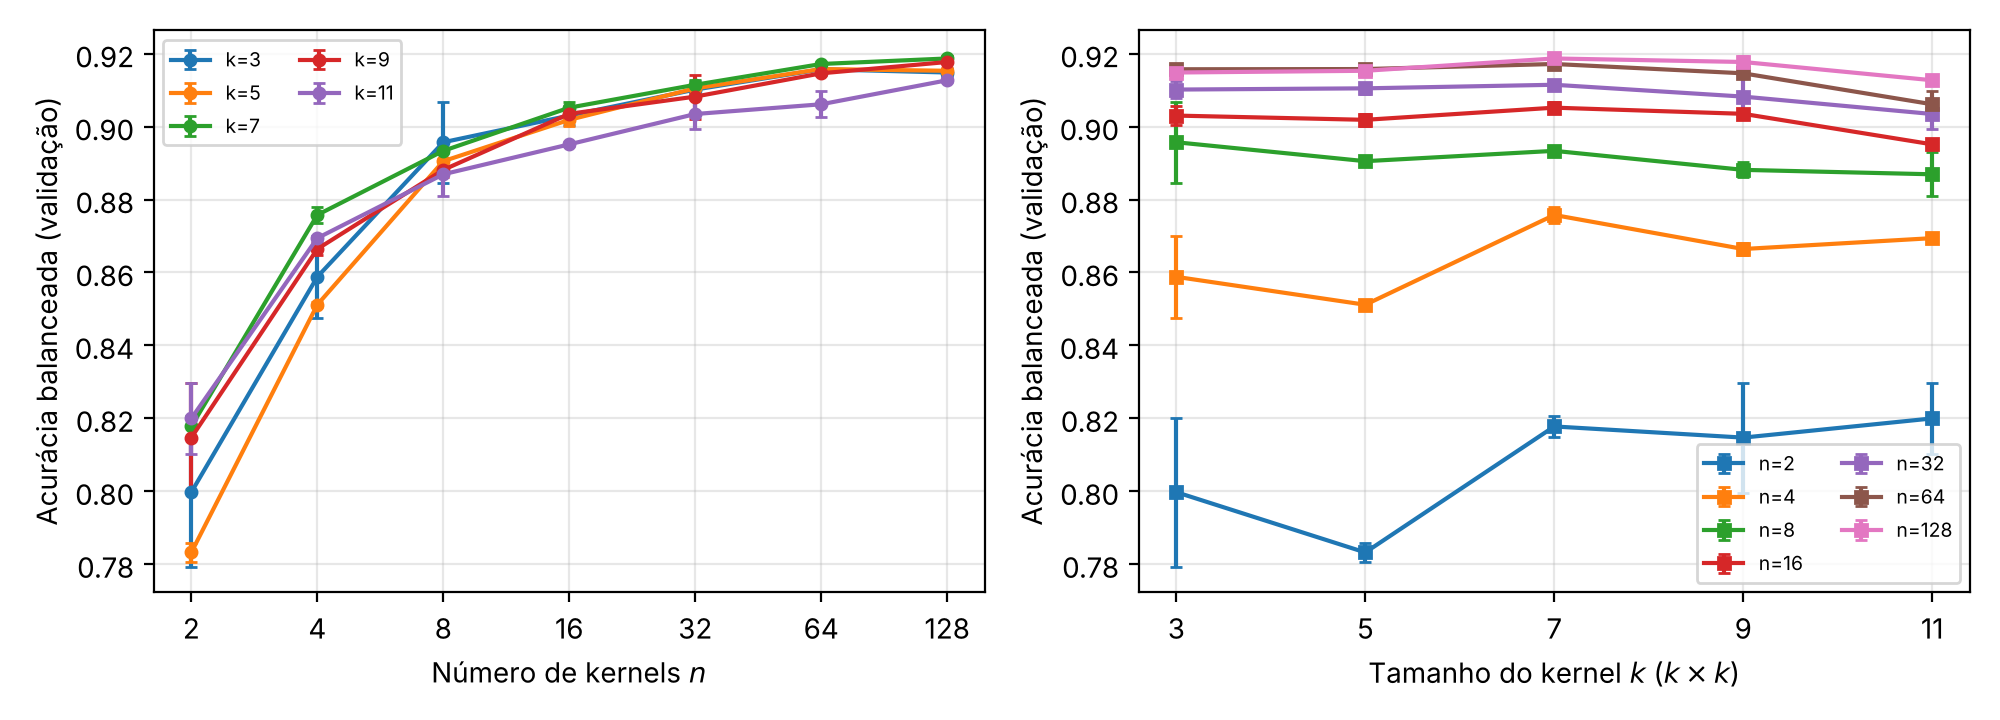
\includegraphics[width=.98\linewidth]{b_progression.png}
\caption{Progressão da BAcc de validação em função de $n$ (esq., escala $\log_2$) e de $k$ (dir.). Barras: desvio entre 2 sementes.}\label{fig:prog}
\end{figure}

\paragraph{Efeito do número de kernels $n$.} É o fator dominante (\cref{fig:prog}, esq.). De $n=2$ para
$n=16$ a BAcc sobe, em média sobre $k$, $\bNgain$ p.p.; a curva é aproximadamente logarítmica (ganhos
decrescentes por duplicação) e satura entre $n=64$ e $128$, onde as diferenças ($<0{,}5$ p.p.) são
comparáveis ao desvio entre sementes. Com poucos kernels a representação é um gargalo de informação: com
$n=2$ a camada densa recebe só 392 atributos, insuficientes para codificar simultaneamente cor e
forma/textura. Note-se também que a BAcc de \emph{treino} cresce de 81--85\% ($n=2$) até 96--100\%
($n=128$, \cref{tab:train}): a partir de $n\approx32$ o modelo aproxima-se da interpolação do treino e o ganho adicional de
validação vem do efeito de regularização implícita de modelos superparametrizados, não de maior ajuste.

\paragraph{Efeito do tamanho do kernel $k$.} É secundário e não monotônico (\cref{fig:prog}, dir.): para
$n\ge16$, $k\in\{3,5,7\}$ ficam praticamente empatados e há uma queda sistemática para $k=11$ (até
$\approx1$ p.p.). Interpretação: (i) com uma única camada convolucional seguida de um \emph{pool} $2\times2$
e de uma camada densa sobre o mapa \emph{inteiro}, a camada de saída já integra informação global, de forma
que campos receptivos grandes na convolução são redundantes; (ii) kernels grandes têm $3k^2$ pesos por filtro
(363 para $k=11$ contra 27 para $k=3$), aumentando a variância de estimação sem ganho de expressividade útil,
e o \emph{padding} com zeros passa a cobrir grande parte do suporte nas bordas. O ótimo em $k=7$ é
compatível com a escala dos grânulos citoplasmáticos e do contorno nuclear (poucos pixels a 28$\times$28).
Para $n$ pequeno ($n\le4$) $k$ maior ajuda ligeiramente, pois cada um dos poucos filtros precisa capturar
mais contexto. O custo de treinamento cresce como $O(nk^2)$ por imagem (\texttt{b\_summary.json}).

\begin{table}[h]
\centering\footnotesize
\caption{BAcc de \emph{treino} (\%) na melhor época de validação: evidência de sobreajuste crescente com $n$.}\label{tab:train}
\begin{tabular}{c|ccccccc}\toprule
$k\backslash n$ & 2 & 4 & 8 & 16 & 32 & 64 & 128\\\midrule
\tabinput{gen/tab_cnn_train.tex}
\bottomrule\end{tabular}
\end{table}

\paragraph{Configuração escolhida.} $n=\bBestN$, $k=\bBestK$: BAcc de validação $\bBestVal\pm\bBestStd\%$,
$\cParams$ parâmetros. Como $(64,7)$ e $(128,9)$ estão a menos de 0,2 p.p., uma escolha guiada por
parcimônia ($n=64$, metade dos parâmetros) seria igualmente defensável; mantivemos o critério objetivo
pré-definido (maior BAcc média de validação).

%======================================================================
\section{(c) Melhor CNN simples: avaliação no teste}\label{sec:cnnc}
%======================================================================
O modelo $(n,k)=(\bBestN,\bBestK)$ foi retreinado com 5 novas sementes (1000--1004), paciência 15 e até 100
épocas (orçamento maior que na varredura, já que agora se trata de um único modelo); o de maior BAcc de
validação ($\cVal\%$) foi avaliado no teste.

\begin{table}[h]
\centering\small
\caption{CNN simples -- desempenho no conjunto de teste.}\label{tab:cnnres}
\begin{tabular}{lcccc}\toprule
 & Acc (\%) & BAcc (\%) & $\Fmac$ (\%) & $F_1^{\mathrm{pond}}$ (\%)\\\midrule
Melhor versão (sel. por validação) & \cAcc & \cBacc & \cFone & \cFw\\
5 sementes (média $\pm$ desvio) & -- & $\cBaccMS$ & $\cFoneMS$ & --\\\bottomrule
\end{tabular}
\end{table}

\begin{figure}[h]
\centering
\begin{subfigure}{.46\linewidth}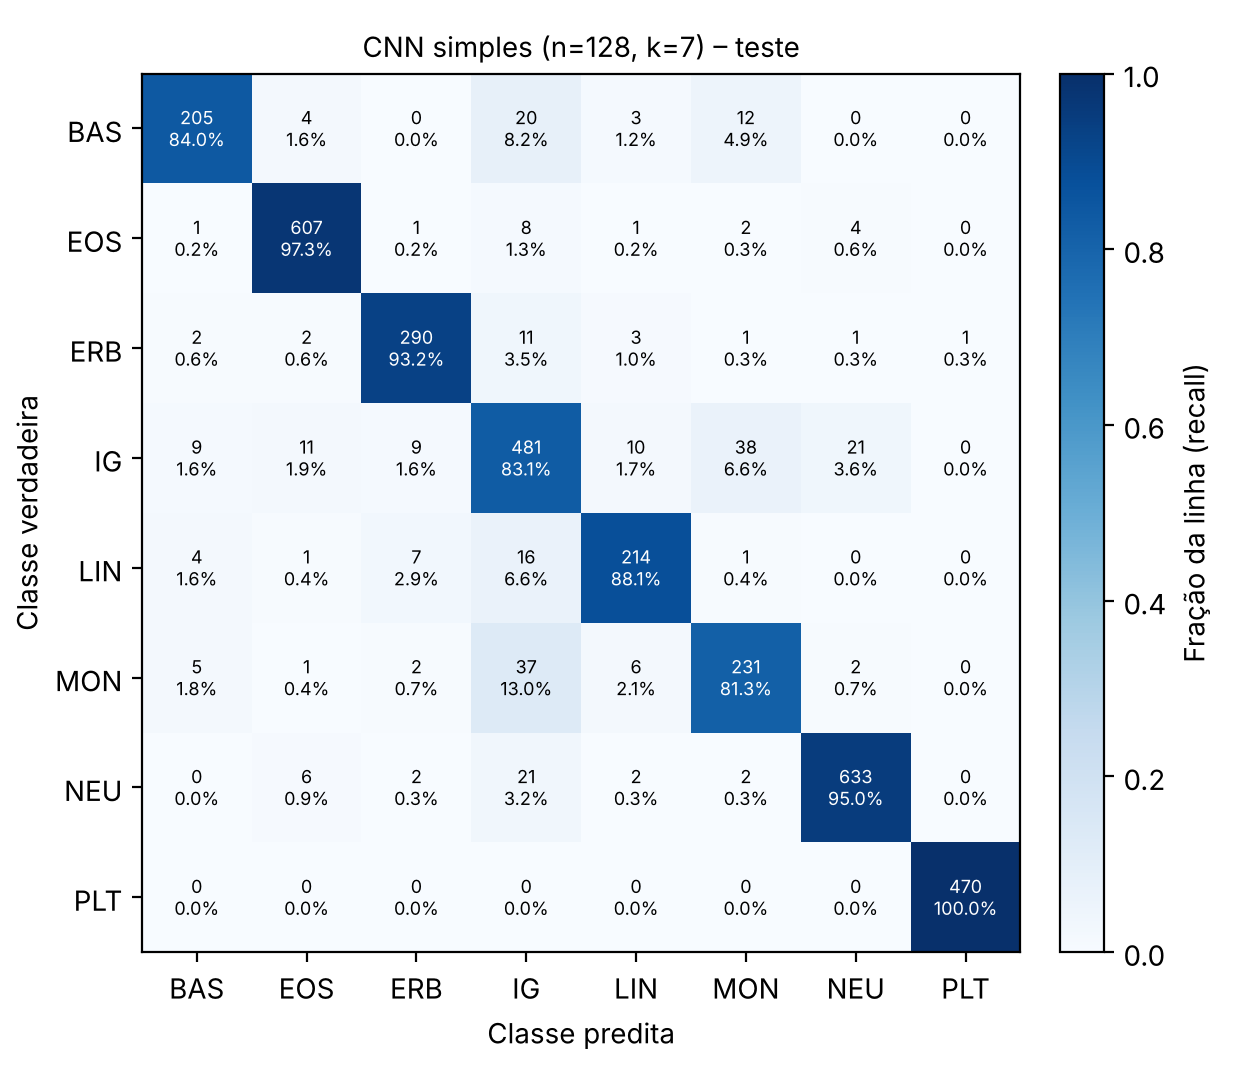
\includegraphics[width=\linewidth]{c_cnn_cm.png}\caption{Matriz de confusão (teste).}\end{subfigure}\hfill
\begin{subfigure}{.52\linewidth}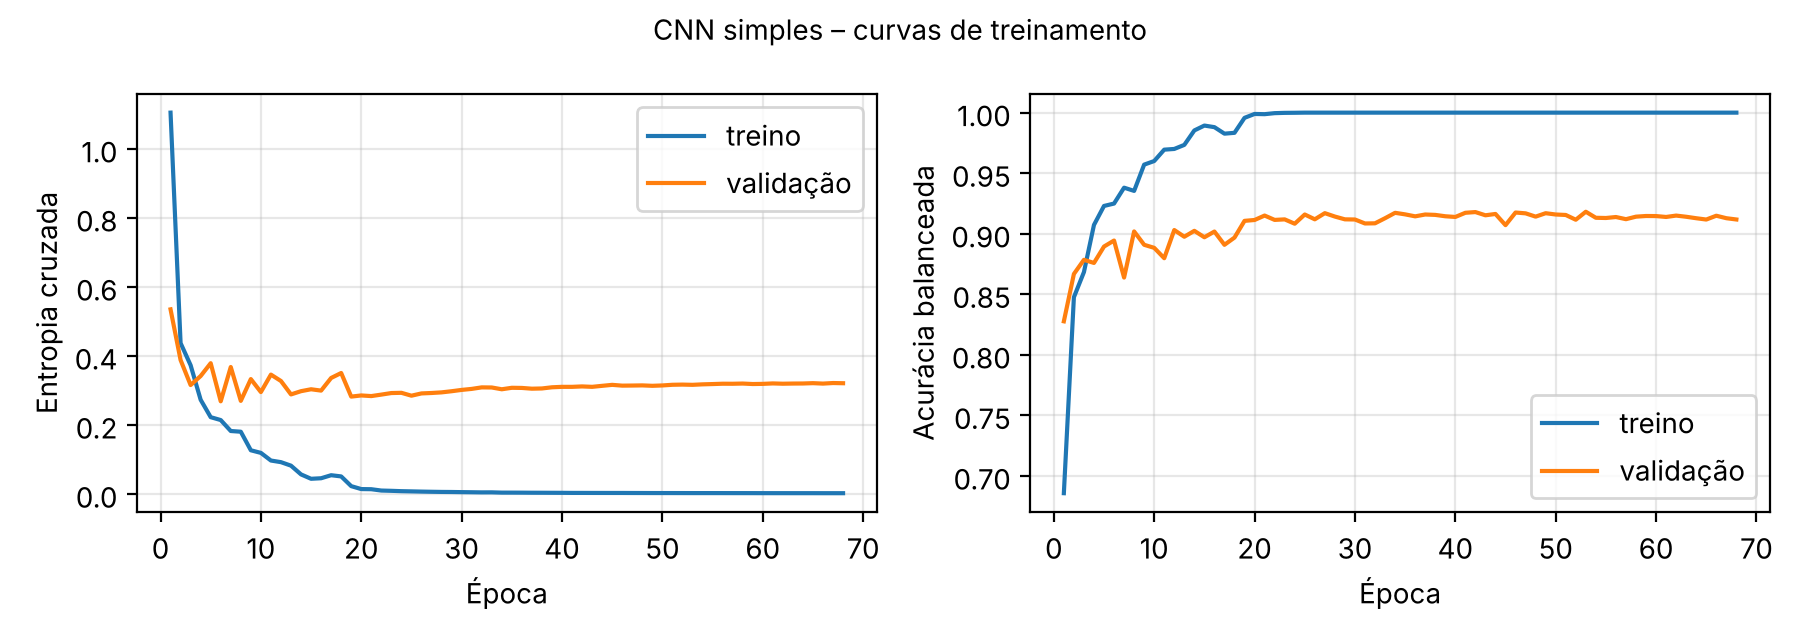
\includegraphics[width=\linewidth]{c_cnn_hist.png}\caption{Curvas de treinamento.}\vspace{2mm}
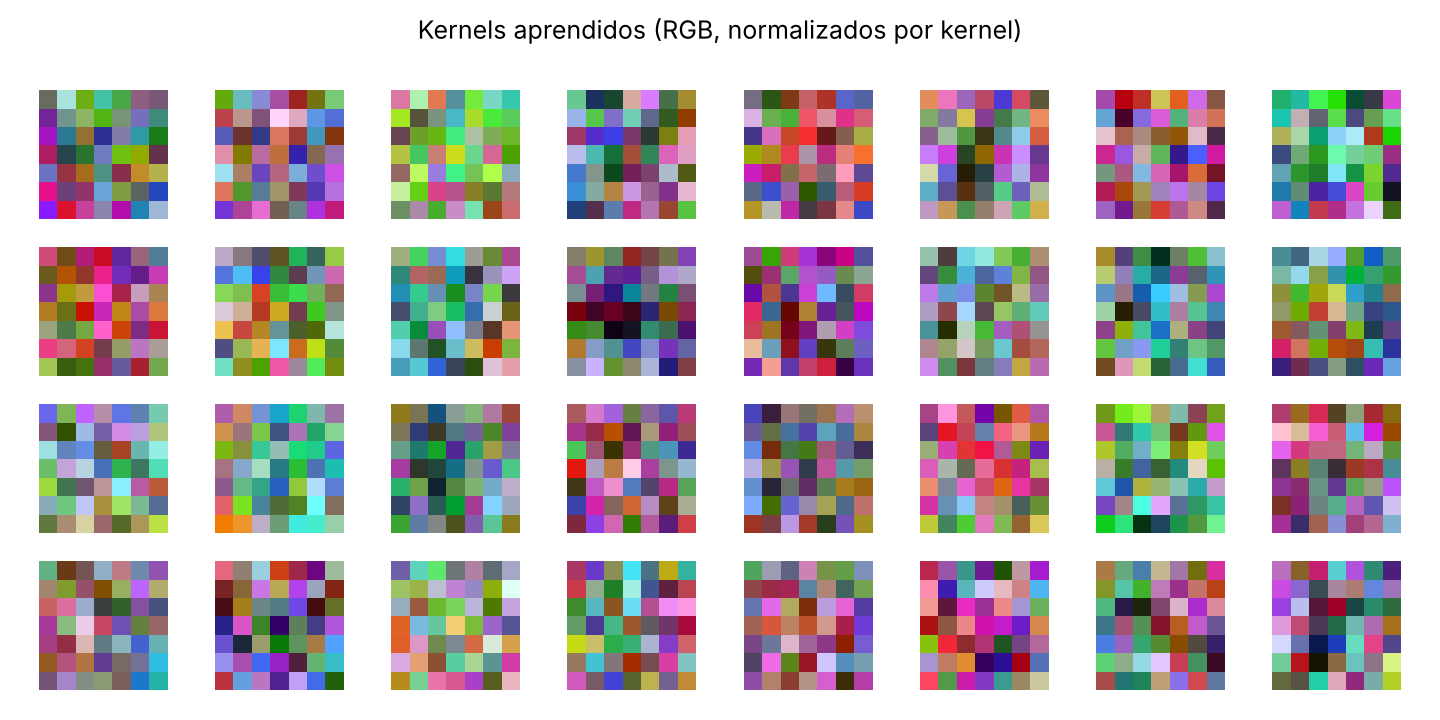
\includegraphics[width=\linewidth]{c_kernels.png}\caption{32 dos 128 kernels $7\times7\times3$ aprendidos.}\end{subfigure}
\caption{CNN simples ($n=\bBestN$, $k=\bBestK$).}\label{fig:cnn}
\end{figure}

\paragraph{Padrões classificados incorretamente.} Dos 3.421 padrões de teste, \cNerr{} foram classificados
incorretamente. Para não mostrar apenas os erros de confiança saturada (que nada informam sobre a
distribuição estimada), os cinco exemplos foram \emph{sorteados} (semente 0) entre todos os erros, impondo
classes verdadeiras distintas (\cref{tab:err,fig:err}).

\begin{table}[h]
\centering\footnotesize\setlength{\tabcolsep}{3.6pt}
\caption{Cinco padrões de teste classificados incorretamente: índice no conjunto de teste, classe esperada,
classe predita e probabilidades $\hat p_c$ estimadas pela softmax. \textcolor{green!45!black}{\textbf{Verde}}:
classe correta; \textcolor{red!70!black}{\textbf{vermelho}}: classe predita.}\label{tab:err}
\begin{tabular}{rcc|cccccccc}\toprule
Índice & Esperada & Predita & BAS & EOS & ERB & IG & LIN & MON & NEU & PLT\\\midrule
\tabinput{gen/tab_errors.tex}
\bottomrule\end{tabular}
\end{table}

\begin{figure}[h]
\centering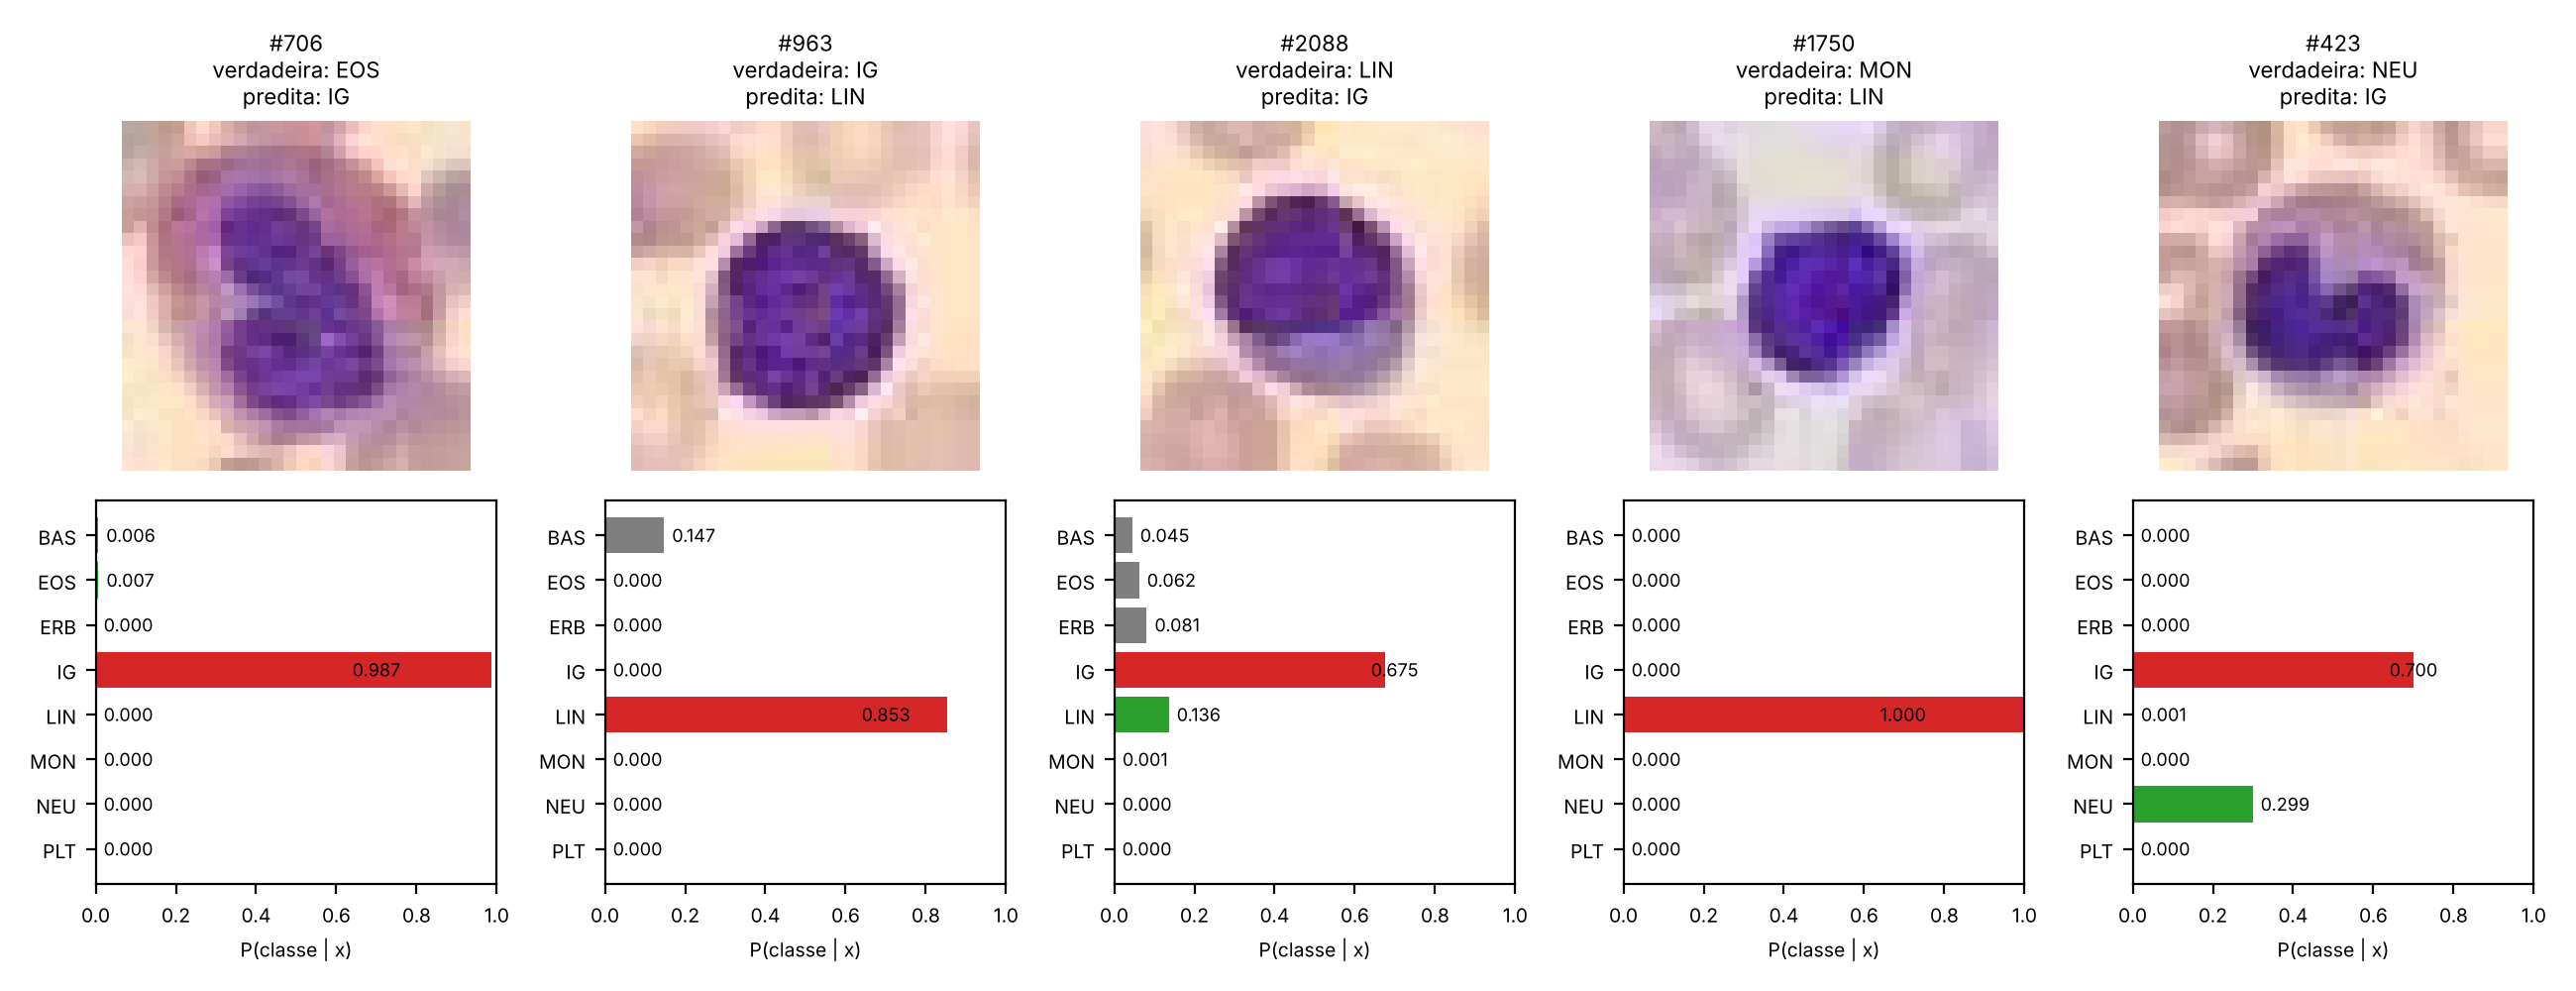
\includegraphics[width=\linewidth]{c_errors.png}
\caption{Os cinco erros da \cref{tab:err}: imagem original $28\times28$ e vetor de probabilidades.}\label{fig:err}
\end{figure}

\paragraph{Discussão.} A CNN de uma única camada convolucional supera a MLP em
$\approx3{,}7$ p.p. de BAcc e $\approx4{,}1$ p.p. de $\Fmac$ (3,4 p.p. na média das 5 sementes) usando \textbf{11 vezes menos parâmetros}
($\cParams$ vs.\ $\mlpParams$), e a diferença é mais de dez vezes maior que o desvio entre sementes de
cada modelo --- logo, é sistemática. Isso quantifica o valor dos vieses indutivos de localidade e
compartilhamento de pesos: os kernels aprendidos (\cref{fig:cnn}c) são, em sua maioria, detectores de
contraste cromático (roxo nuclear $\times$ rosa citoplasmático $\times$ fundo) e de bordas orientadas, aplicados
em qualquer posição. As maiores melhorias por classe ocorreram justamente nas classes morfologicamente
difíceis: BAS (75,0\%$\to$84,0\% de revocação) e IG (72,5\%$\to$83,1\%). O padrão residual de confusão,
porém, é o mesmo da MLP: a coluna IG é o principal ``sumidouro'' de erros (13,0\% dos MON, 8,2\% dos BAS,
6,6\% dos LIN e 3,2\% dos NEU), refletindo a heterogeneidade intrínseca dessa classe.

Os exemplos ilustram três tipos de falha:
(i) \emph{ambiguidade morfológica genuína} --- \#2088 (LIN$\to$IG) e \#423 (NEU$\to$IG) têm distribuições
não degeneradas, com a classe correta em 2º lugar (0,136 e 0,299); o neutrófilo \#423 tem núcleo em ``ferradura''
pouco segmentado, típico de bastonete/metamielócito, i.e., na fronteira com IG;
(ii) \emph{perda de informação pela resolução} --- no eosinófilo \#706 os grânulos alaranjados são pouco
visíveis a $28\times28$ e o núcleo alongado possivelmente lembra o de um IG; (iii) \emph{erros de alta confiança} --- \#1750
(MON$\to$LIN, $\hat p=1{,}000$) é um monócito pequeno com núcleo compacto e pouca margem citoplasmática visível,
fenótipo que, nessa resolução, é indistinguível de um linfócito.

O caso (iii) não é isolado: a mediana da confiança $\max_c\hat p_c$ nos erros é \cConfErr{} e
$\cFracHigh\%$ dos erros têm confiança $>0{,}9$, contra mediana \cConfOk{} nos acertos; a probabilidade
atribuída à classe correta nos erros tem mediana \cPtrue{}, embora ela esteja entre as duas mais prováveis em
$\cTopTwo\%$ dos erros. O erro esperado de calibração é ECE $=\cECE$ (15 \emph{bins}). Trata-se do conhecido
excesso de confiança de redes treinadas até interpolar o treino (BAcc de treino $\approx100\%$,
\cref{tab:train}); em uso clínico, recomendar-se-ia calibração pós-treino (p.ex., \emph{temperature scaling} \cite{guo2017}
na validação) antes de usar $\hat p$ como grau de certeza.

%======================================================================
\section{(d) Transfer learning com ResNet-18 pré-treinada}\label{sec:tl}
%======================================================================
\paragraph{Modelo-base e adaptação da saída.} ResNet-18 \cite{he2016} (\texttt{torchvision.models.resnet18},
11,2 M parâmetros), escolhida por ser uma CNN residual canônica, com pesos ImageNet-1k amplamente disponíveis e
custo compatível com treinamento em CPU. Os pesos ImageNet-1k carregados são os
\texttt{resnet18.a1\_in1k} (receita ``ResNet strikes back'' \cite{wightman2021}), distribuídos em formato
\texttt{state\_dict} idêntico ao do \texttt{torchvision}\footnote{No ambiente de execução, o servidor de pesos
do \texttt{torchvision} estava inacessível; o script aceita qualquer \texttt{state\_dict} compatível via
\texttt{-{}-weights} e, sem esse argumento, usa \texttt{weights="IMAGENET1K\_V1"} do \texttt{torchvision}.}.
A camada \texttt{fc} ($512\to1000$) foi substituída por $\mathrm{Dropout}(0{,}2)\to\mathrm{Linear}(512\to8)$,
inicializada aleatoriamente; todo o restante foi herdado.

\paragraph{Adaptação da entrada.} Com $28\times28$, o tronco da ResNet (conv $7\times7$/2 + \emph{max-pool}/2)
reduziria a imagem a $7\times7$ antes do primeiro bloco e a $1\times1$ no último estágio, destruindo a
informação espacial. As imagens são então interpoladas bilinearmente para $\ftSize\times\ftSize$ (mapa final
$2\times2$), compromisso entre preservar a hierarquia espacial para a qual os pesos foram aprendidos e o custo
computacional em CPU ($\approx$4$\times$ mais barato que $128\times128$).

\paragraph{Aumentação.} Apenas transformações do grupo diedral $D_4$ (\emph{flips} horizontal/vertical e
transposição, gerando as 8 rotações/reflexões de $90^\circ$): células em esfregaço não têm orientação
canônica, logo o rótulo é exatamente invariante a $D_4$, e essas transformações não exigem interpolação
(sem artefatos). Alterações de cor foram evitadas por a coloração ser informação discriminativa (EOS, BAS).

\paragraph{Validação cruzada.} Uniram-se treino e validação oficiais (13.671 imagens) e aplicou-se
validação cruzada estratificada com $K=\ftK$ partições (semente 0), mantendo o \textbf{teste oficial
intocado}. A CV foi usada para (i) comparar duas estratégias de transferência com estimativa de variância e
(ii) obter $K$ modelos para avaliação individual e em comitê:
\begin{itemize}
\item \textbf{FE (extração de atributos)}: tronco congelado; atributos de 512 dimensões (após \emph{global
average pooling}) pré-computados, padronizados com estatísticas da partição de treino do \emph{fold}, e apenas
a cabeça treinada (Adam, $\le200$ épocas, paciência 20);
\item \textbf{FT (ajuste fino completo)}: todos os pesos treinados com AdamW (\emph{weight decay} 0,05),
taxas discriminativas --- $10^{-3}$ na cabeça e $10^{-4}$ no tronco, para não destruir os atributos
pré-treinados nas primeiras iterações, quando o gradiente da cabeça aleatória é ruidoso ---, cronograma
cosseno em $\ftEpochs$ épocas, lotes de 64, CE ponderada com \emph{label smoothing} 0,05 e restauração
da época de melhor BAcc no \emph{fold} de validação.
\end{itemize}

\begin{table}[h]
\centering\footnotesize\setlength{\tabcolsep}{4pt}
\caption{Validação cruzada estratificada ($K=\ftK$) e desempenho de cada modelo de \emph{fold} no teste.}\label{tab:cv}
\begin{tabular}{c|ccc|cccc}\toprule
 & \multicolumn{3}{c|}{BAcc no \emph{fold} de validação} & \multicolumn{4}{c}{FT -- teste oficial}\\
\emph{Fold} & FT (\%) & melhor época & FE (\%) & Acc (\%) & BAcc (\%) & $\Fmac$ (\%) & tempo (min)\\\midrule
\tabinput{gen/tab_cv.tex}\midrule
Média $\pm$ desvio & \multicolumn{2}{c}{$\ftCV$} & $\feCV$ & $\ftFoldAccMS$ & $\ftFoldBaccMS$ & $\ftFoldFoneMS$ & \ftFoldTime\\
\bottomrule\end{tabular}
\end{table}

\begin{table}[h]
\centering\small
\caption{ResNet-18 -- métricas globais no teste (comitê = média das probabilidades dos \ftK{} modelos de \emph{fold}).}\label{tab:tlres}
\begin{tabular}{lcccc}\toprule
 & Acc (\%) & BAcc (\%) & $\Fmac$ (\%) & $F_1^{\mathrm{pond}}$ (\%)\\\midrule
FE (tronco congelado), comitê & \feAcc & \feTest & \feFone & --\\
FT, modelo individual (média $\pm$ desvio) & $\ftFoldAccMS$ & $\ftFoldBaccMS$ & $\ftFoldFoneMS$ & --\\
FT, comitê de \ftK{} modelos & \ftEnsAcc & \ftEnsBacc & \ftEnsFone & \ftEnsFw\\\bottomrule
\end{tabular}
\end{table}

\begin{figure}[h]
\centering
\begin{subfigure}{.46\linewidth}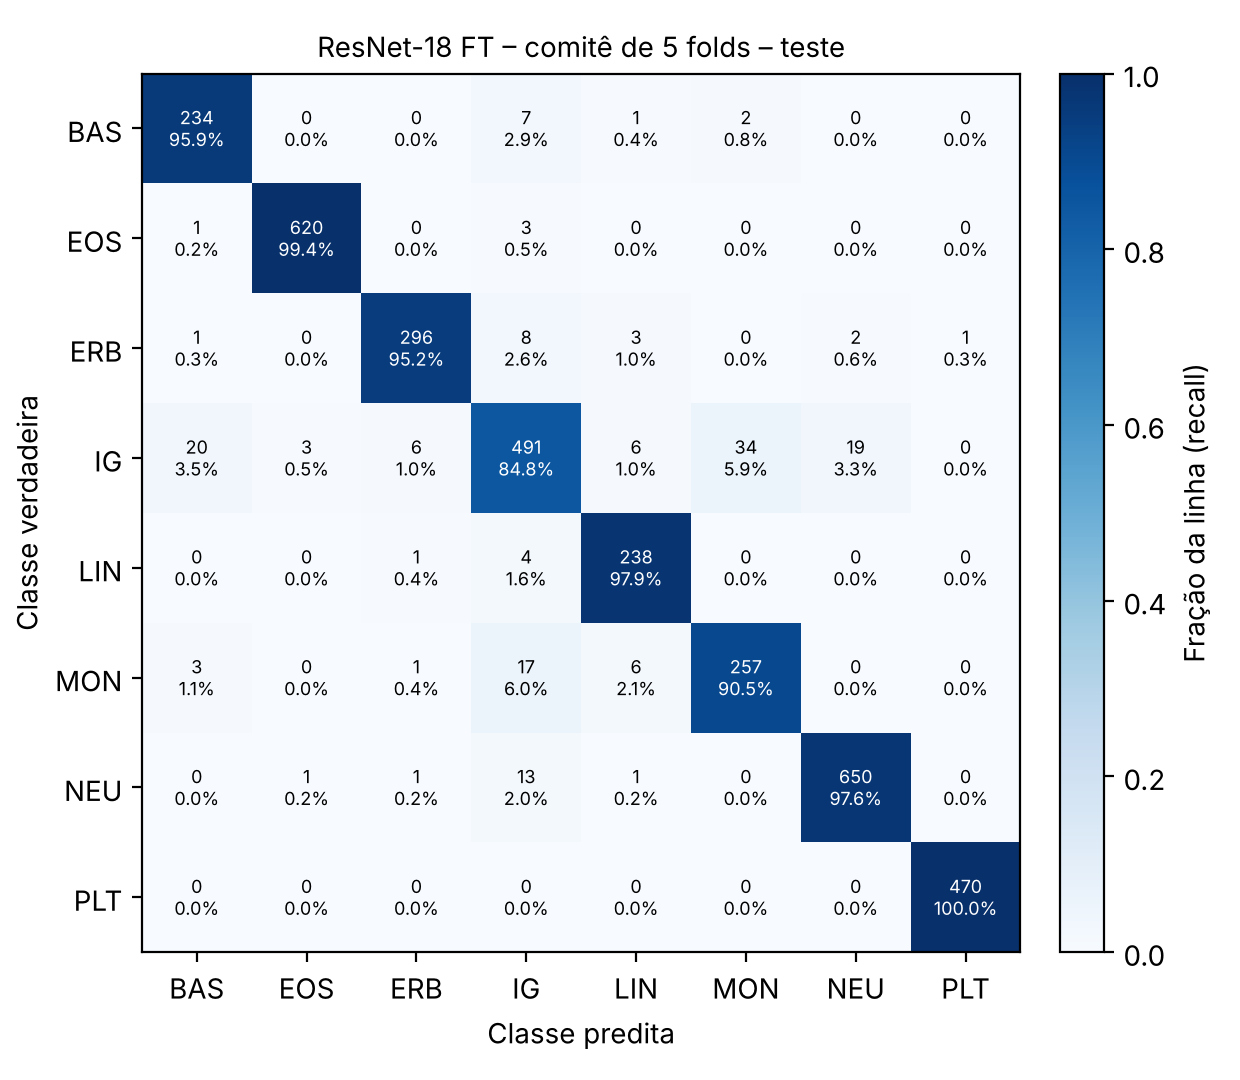
\includegraphics[width=\linewidth]{d_ft_cm_ensemble.png}\caption{Comitê FT (teste).}\end{subfigure}\hfill
\begin{subfigure}{.46\linewidth}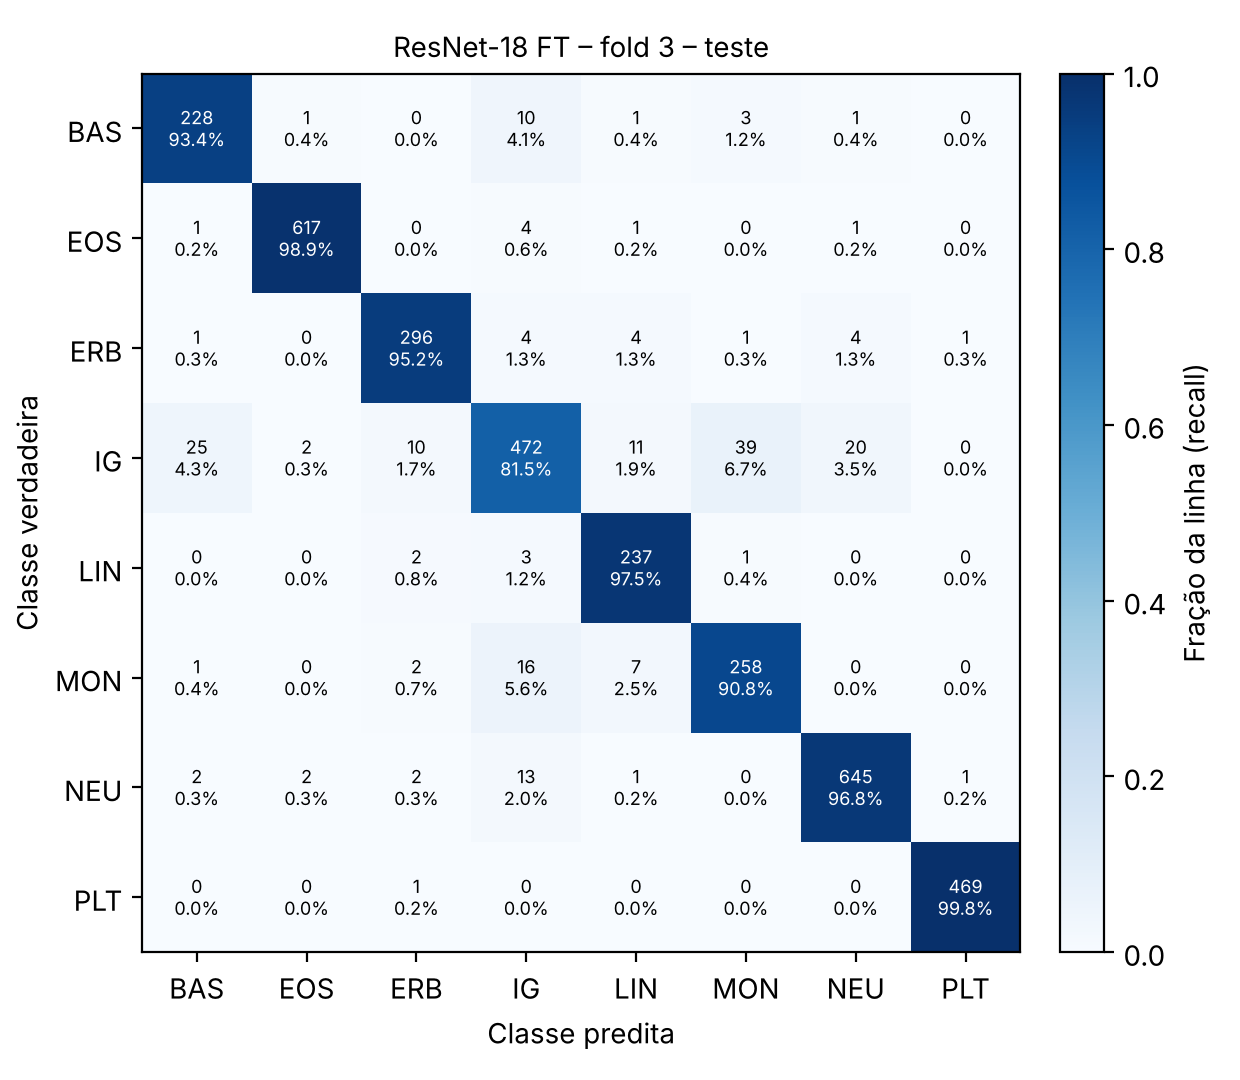
\includegraphics[width=\linewidth]{d_ft_cm_single.png}\caption{Melhor \emph{fold} individual (teste).}\end{subfigure}
\caption{Matrizes de confusão da ResNet-18 com ajuste fino.}\label{fig:tlcm}
\end{figure}

\paragraph{Discussão.}
\textbf{(i) Extração de atributos falha; ajuste fino é essencial.} Com o tronco congelado, a BAcc na CV foi
de apenas $\feCV\%$ e $\feTest\%$ no teste --- \emph{abaixo da MLP} treinada do zero. Os atributos da última
camada de uma rede treinada na ImageNet codificam semântica de objetos naturais, e o domínio aqui é muito
distinto: imagens de microscopia com coloração de May--Grünwald--Giemsa, objeto único centrado e,
sobretudo, imagens de $28\times28$ interpoladas, sem as altas frequências que os filtros iniciais da rede esperam.
Uma cabeça linear sobre esses 512 atributos não consegue reconstruir as pistas finas (granulação, cromatina)
que separam IG, MON e BAS. Já o ajuste fino completo atinge $\ftCV\%$ na CV: a transferência é útil
como \emph{inicialização} --- filtros genéricos de borda/textura e um ponto de partida bem condicionado para
uma rede profunda ---, não como extrator fixo. Dada a diferença de $\approx15$ p.p. entre as estratégias,
muito maior que os desvios entre \emph{folds} ($<1$ p.p.), a escolha de FT pela CV é inequívoca.

\textbf{(ii) Estabilidade e generalização.} O desvio entre \emph{folds} é pequeno ($0{,}36$ p.p. na CV e
$0{,}25$ p.p. no teste), indicando baixa sensibilidade à partição. A BAcc média no teste
($\ftFoldBaccMS\%$) ficou ligeiramente \emph{acima} da estimativa por CV ($93{,}77\%$); como cada
\emph{fold} de validação tem apenas $\approx2.700$ imagens (e $\approx195$ basófilos), a diferença está dentro
do erro de estimação, e não há sinal de sobreajuste à seleção. O comitê dos 5 modelos (média das
probabilidades) acrescenta $+0{,}76$ p.p. de BAcc ($\ftEnsBacc\%$), efeito típico de redução de variância por
\emph{ensembling}, ao custo de $5\times$ mais parâmetros e tempo de inferência.

\textbf{(iii) Estrutura dos erros.} A matriz de confusão do comitê (\cref{fig:tlcm}) mantém
o padrão qualitativo das redes anteriores, porém muito atenuado: IG continua sendo a classe mais difícil
(84,8\% de revocação; confunde-se com MON, BAS e NEU) e MON a segunda (90,5\%, com 6,0\% previstos como IG).
Os basófilos, que eram o ponto fraco da MLP (75,0\%), chegam a 95,9\%, e LIN a 97,9\%. As classes com
assinatura cromática forte (EOS, PLT) ficam próximas de 100\%.

\textbf{(iv) Treinamento ainda não saturado.} A melhor época foi a 10ª--12ª em todos os \emph{folds}, com a
BAcc de validação ainda crescendo lentamente sob o cronograma cosseno; o orçamento de 12 épocas e a resolução
$64\times64$ foram impostos pelo uso exclusivo de CPU ($\approx\ftEpochTime$ s/época). Para referência, o
\emph{benchmark} oficial \cite{yang2021} reporta acurácia de 95,8\% para a ResNet-18 treinada
por 100 épocas (Adam) em $28\times28$ e 96,3\% com entradas redimensionadas para $224\times224$; nosso comitê
(Acc $=\ftEnsAcc\%$) e os modelos individuais ($\ftFoldAccMS\%$) estão nessa faixa, e é razoável esperar
ganhos adicionais com mais épocas e maior resolução de entrada em GPU.


%======================================================================
\section{Comparação geral: MLP $\times$ CNN artesanal $\times$ CNN com \emph{transfer learning}}\label{sec:cmp}
%======================================================================
\begin{table}[h]
\centering\footnotesize\setlength{\tabcolsep}{4pt}
\caption{Comparação no teste oficial. ``Média $\pm$ desvio'': entre sementes (MLP, CNN) ou entre
\emph{folds} (ResNet). Tempo de treinamento: modelo selecionado (para o comitê, soma dos \ftK{} \emph{folds});
inferência: 3.421 imagens de teste, CPU 2 núcleos.}\label{tab:cmp}
\begin{tabular}{lrcccccc}\toprule
Modelo & Parâmetros & Acc (\%) & BAcc (\%) & $\Fmac$ (\%) & BAcc ($\mu\pm\sigma$) & Treino (min) & Infer. (s)\\\midrule
\tabinput{gen/tab_compare.tex}
\bottomrule\end{tabular}
\end{table}

\begin{figure}[h]
\centering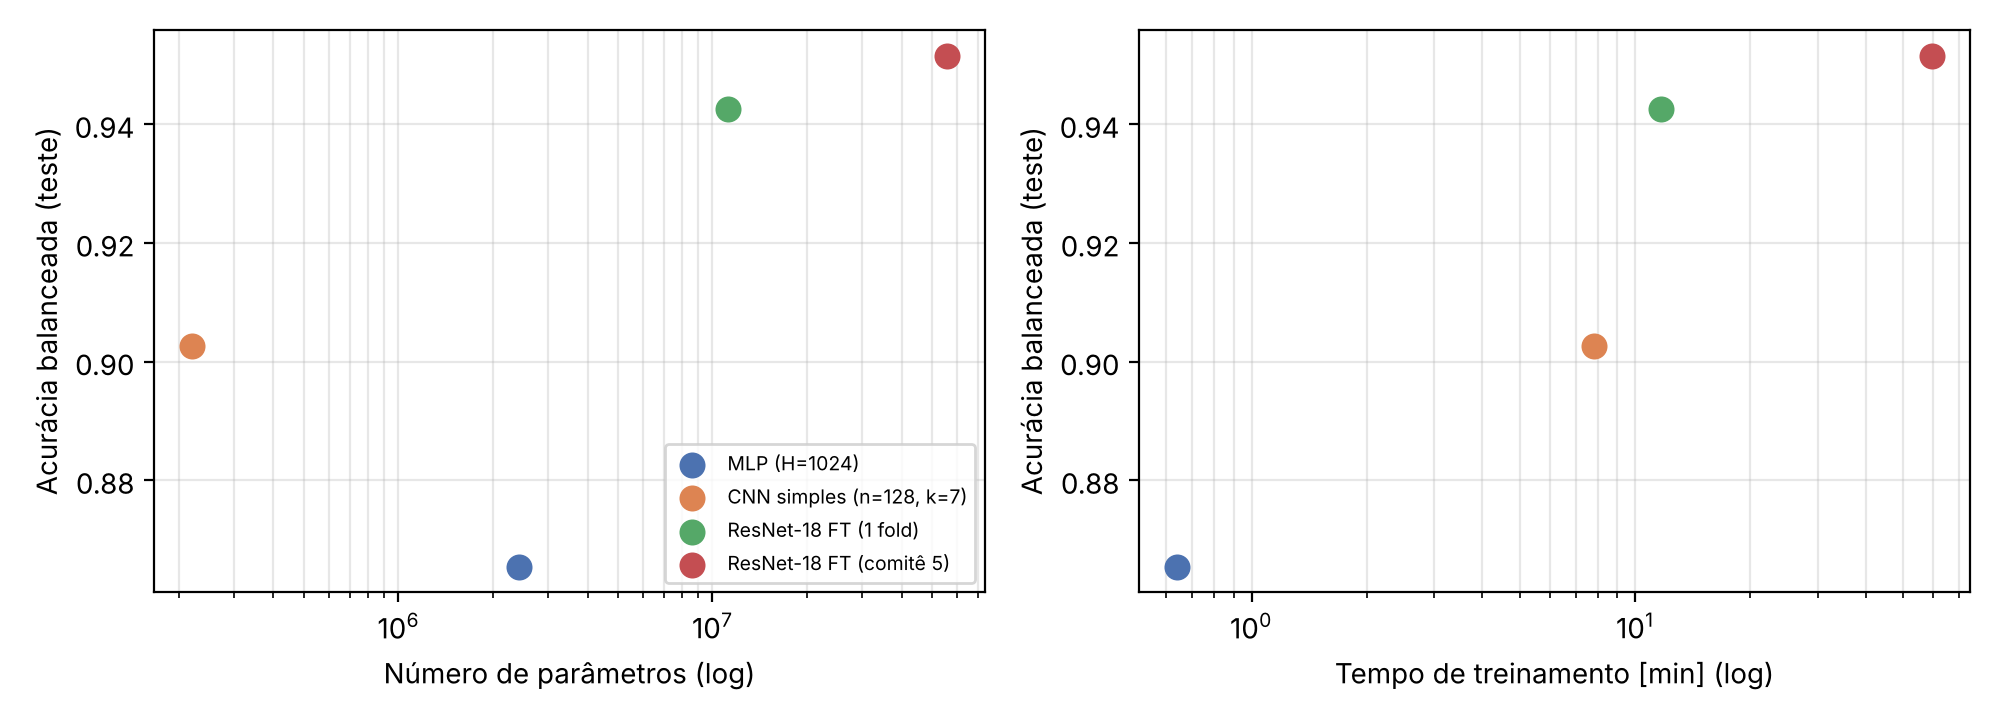
\includegraphics[width=.95\linewidth]{e_compare.png}
\caption{BAcc de teste versus número de parâmetros (esq.) e tempo de treinamento (dir.), escalas logarítmicas.}\label{fig:cmp}
\end{figure}

\begin{table}[h]
\centering\small
\caption{$F_1$ por classe no teste (\%). Em negrito, o melhor modelo para cada classe.}\label{tab:f1pc}
\begin{tabular}{lcccc}\toprule
Classe & MLP & CNN simples & ResNet-18 FT & ResNet-18 FT (comitê)\\\midrule
\tabinput{gen/tab_f1pc.tex}
\bottomrule\end{tabular}
\end{table}

\paragraph{Desempenho.} A ordenação MLP $<$ CNN artesanal $<$ ResNet-18 é estrita em todas as métricas
globais (\cref{tab:cmp}) e as diferenças são grandes frente à variabilidade observada (desvios de
0,17--0,25 p.p. entre sementes/\emph{folds}): $+3{,}7$ p.p. de BAcc da MLP para a CNN simples e $+4{,}0$ p.p. da
CNN simples para uma única ResNet-18 ajustada (+4,9 p.p. com o comitê). Por classe (\cref{tab:f1pc}), os
ganhos concentram-se nas classes morfologicamente próximas --- BAS ($F_1$: 74,5 $\to$ 87,2 $\to$ 93,0\%),
MON (76,5 $\to$ 80,9 $\to$ 89,1\%) e IG (74,7 $\to$ 82,0 $\to$ 87,5\%) ---, enquanto EOS, NEU e PLT, separáveis
essencialmente por cor e tamanho, já estão acima de 93\% mesmo na MLP. Ou seja, cada salto de
arquitetura compra discriminação de \emph{forma/textura}: localidade e compartilhamento de pesos (CNN
simples) e, depois, hierarquia profunda de atributos com inicialização pré-treinada (ResNet).

\paragraph{Parâmetros.} O número de parâmetros \emph{não} explica o desempenho por si só: a CNN simples tem
11$\times$ \emph{menos} parâmetros que a MLP e é melhor, porque 99,5\% dos parâmetros da MLP estão na matriz
$2352\times1024$ que liga cada pixel a cada neurônio sem nenhuma estrutura, enquanto a CNN gasta só 18.944
parâmetros na convolução (compartilhados por todas as posições) e o restante na camada de saída. A ResNet-18
tem 51$\times$ mais parâmetros que a CNN simples e 4,6$\times$ mais que a MLP, mas eles estão
organizados em 17 camadas convolucionais principais com conexões residuais e, sobretudo, \emph{não partem do zero}: o
pré-treino funciona como um forte \emph{prior} que permite usar essa capacidade com apenas $\approx11$ mil
imagens sem sobreajuste severo. Em termos de custo computacional, a métrica relevante é o número de
multiplicações-acumulações por imagem: $\approx2{,}4$\,M (MLP), $\approx15{,}0$\,M (CNN simples, quase toda
na convolução $28\times28\times128\times147$) e $\approx148$\,M (ResNet-18 a $64\times64$), o que se reflete
na inferência sobre o teste: 0,06\,s, 1,5\,s e 4,3\,s, respectivamente (CPU).

\paragraph{Tempo de treinamento.} Treinar o modelo final levou 0,6\,min (MLP), 7,8\,min (CNN simples,
68 épocas; média de 5,4\,min entre sementes) e 11,7\,min por \emph{fold} da ResNet-18 (12 épocas de
$\approx\ftEpochTime$\,s), ou $\ftTotalTime$\,min para a CV completa. O custo da \emph{seleção de modelo}, porém,
inverte parcialmente essa ordem: a busca da MLP custou $\approx17$\,min (30 treinamentos), a varredura da CNN
$\approx\bTotalTime$\,min (70 treinamentos) e a ResNet dispensou busca extensa de arquitetura --- a CV
foi usada para escolher entre duas estratégias de transferência e, ao mesmo tempo, produziu os 5 modelos do
comitê. Por época, a ResNet é $\approx9\times$ mais lenta que a CNN simples ($\approx7$\,s/época), mas converge
em muito menos épocas graças ao pré-treino (BAcc de validação de 90,5--92,2\% já na 4ª época).

\paragraph{Compromisso.} Se o critério for exclusivamente desempenho, a ResNet-18 ajustada (preferencialmente
em comitê) é a escolha clara: reduz o erro balanceado de 9,7\% (CNN simples) para 4,8\%, i.e., à metade. Se
houver restrição severa de memória/energia (p.ex., embarcado), a CNN simples oferece $\approx95\%$ do
desempenho da ResNet com 2\% dos parâmetros e 10\% das operações. A MLP é dominada: é pior que a CNN em
desempenho e em número de parâmetros, vencendo apenas em custo de operações --- irrelevante nesta escala.

\section{Conclusões}
\begin{itemize}
\item A MLP de uma camada oculta ($H=1024$, ReLU, BN, dropout 0,25, CE ponderada) atinge BAcc $=\mlpBacc\%$ e
$\Fmac=\mlpFone\%$ no teste; os erros concentram-se no grupo BAS--IG--MON, que exige informação espacial.
\item Na CNN simples, o número de kernels é o fator dominante (ganho logarítmico com saturação em $n\approx64$--128);
o tamanho do kernel tem efeito pequeno, com ótimo em $k=7$ e degradação para $k=11$. A melhor configuração
($n=\bBestN$, $k=\bBestK$) obtém BAcc $=\cBacc\%$ e $\Fmac=\cFone\%$ com 11$\times$ menos parâmetros que a MLP,
mas é excessivamente confiante nos erros (ECE $=\cECE$).
\item A ResNet-18 pré-treinada só é vantajosa com ajuste fino completo (FE: $\feTest\%$; FT: $\ftFoldBaccMS\%$
por modelo e $\ftEnsBacc\%$ em comitê), resultado compatível com o \emph{benchmark} MedMNIST v2 mesmo sob
orçamento de CPU (12 épocas, $64\times64$).
\item Granulócitos imaturos permanecem a classe mais difícil para todos os modelos, o que é coerente com
o fato de a classe agregar três estágios de maturação morfologicamente contíguos às demais classes.
\end{itemize}


%======================================================================
\section{Reprodutibilidade: organização do código}
%======================================================================
\begin{lstlisting}
common.py           # dados, normalizacao, laco de treino + early stopping, metricas, graficos
a_mlp.py            # item (a): busca em 2 etapas + 5 sementes -> results/a_mlp.json
b_cnn_sweep.py      # item (b): grade n x k, 2 sementes (retomavel) -> results/b_summary.json
c_cnn_best.py       # item (c): retreino da melhor CNN, erros, calibracao -> results/c_cnn.json
d_transfer.py       # item (d): ResNet-18, CV estratificada 5-fold, FE x FT -> results/d_transfer.json
e_compare.py        # comparacao geral -> results/compare.json + figuras
f_dataset_overview.py, gen_tex.py   # figura da base; tabelas/macros LaTeX a partir dos JSONs
run_all.sh          # executa tudo em sequencia:  DATA=data/bloodmnist.npz ./run_all.sh
\end{lstlisting}
Todas as tabelas numéricas deste relatório são geradas automaticamente a partir dos arquivos JSON de
resultados por \texttt{gen\_tex.py}, eliminando transcrição manual.

\begin{thebibliography}{9}\small
\bibitem{yang2021} J. Yang, R. Shi, D. Wei, Z. Liu, L. Zhao, B. Ke, H. Pfister, B. Ni. MedMNIST v2: A
Large-Scale Lightweight Benchmark for 2D and 3D Biomedical Image Classification. \emph{arXiv:2110.14795}, 2021
(publicado em \emph{Scientific Data}, 10:41, 2023).
\bibitem{acevedo2020} A. Acevedo, A. Merino, S. Alférez, A. Molina, L. Boldú, J. Rodellar. A dataset of
microscopic peripheral blood cell images for development of automatic recognition systems. \emph{Data in Brief},
30:105474, 2020.
\bibitem{he2016} K. He, X. Zhang, S. Ren, J. Sun. Deep Residual Learning for Image Recognition. \emph{CVPR}, 2016.
\bibitem{wightman2021} R. Wightman, H. Touvron, H. Jégou. ResNet strikes back: An improved training procedure in
timm. \emph{arXiv:2110.00476}, 2021.
\bibitem{guo2017} C. Guo, G. Pleiss, Y. Sun, K. Q. Weinberger. On Calibration of Modern Neural Networks.
\emph{ICML}, 2017.
\end{thebibliography}
\end{document}
